\documentclass[10pt,a4paper]{article}

\usepackage[utf8]{inputenc}
\usepackage[italian]{babel}
\usepackage{amsmath}
\usepackage{amsfonts}
\usepackage{amssymb}
\usepackage{graphicx}

\usepackage[left=2cm,right=2cm,top=2cm,bottom=2cm]{geometry}
\geometry{a4paper}

\usepackage{booktabs} % for much better looking tables
\usepackage{verbatim}
\usepackage{subfig} % make it possible to include more than one captioned figure/table in a single 

\usepackage{fancyhdr} % This should be set AFTER setting up the page geometry
\pagestyle{fancy} % options: empty , plain , fancy
\renewcommand{\headrulewidth}{0pt} % customise the layout...
\lhead{}\chead{}\rhead{}
\lfoot{}\cfoot{\thepage}\rfoot{}

%%% SECTION TITLE APPEARANCE
\usepackage{sectsty}
%\allsectionsfont{\sffamily\mdseries\upshape} % (See the fntguide.pdf for font help)
% (This matches ConTeXt defaults)

% pacchetti che mi piacciono
\usepackage[cdot, thickqspace]{SIunits}

\title{Esercitazione 2: Circuito RC - Filtri passivi}
\author{Gruppo BE \\ Alessandro Candido, Roberto Ribatti}
\date{\today} 

\begin{document}
\maketitle

\section{Scopo e strumentazione}
Lo scopo dell'esperienza è:
\begin{itemize}
\item verificare il comportamento in frequenza dei filtri RC posti singolarmente e a cascata (l'uscita dell'uno connessa con l'ingresso dell'altro);
\item dimensionare opportunamente un filtro passa-basso al fine di migliorare il rapporto segnale rumore in un caso dato.
\end{itemize}

In particolare per quanto riguarda il primo punto si è analizzato un filtro passa-basso e una configurazione a cascata, in cui il primo stadio era un passa-basso e il secondo un passa-alto. Per il secondo punto si aveva un segnale a $\unit{2}{\kilo\hertz}$ e il rumore a $\unit{20}{\kilo\hertz}$, e si considerava un carico a valle di $\sim \unit{100}{\kilo\ohm}$.

La strumentazione usata è quella presente sul banco di lavoro.
%così suona altamente poco riproducibile, ma dobbiamo trovare una formula per evitare di ripetere ogni volta l'elenco stupido di oscilloscopio, alimentatore, etc.

\section{Filtro passa-basso}

\subsection{Dimensionamento}
Si è dimensionato il circuito tenendo conto dei seguenti criteri:
\begin{itemize}
\item massimizzare il rapporto segnale-rumore;
\item ottenere un segnale abbastanza intenso.
\end{itemize}
Cercare di preservare l'intensità del segnale in ingresso è motivato dal fatto che, se il segnale venisse troppo attenuato dal filtro, gli strumenti per misurarlo introdurrebbero essi stessi un rumore non trascurabile, o comunque sarebbero non trascurabili altri tipi di contributi.

A questo fine si è fissata la frequenza di taglio a $\unit{200}{\hertz}$, infatti minore è la frequenza di taglio maggiore è il rapporto segnale rumore, per cui si otterrebbe un rapporto massimo per una frequenza di taglio nulla. Ma in questo modo si attenuerebbe eccessivamente il segnale, non rispettando il secondo criterio.

A $\unit{200}{\hertz}$ infatti il guadagno è $\sim \unit{-20}{\deci\bel}$ per il segnale, per cui un segnale in ingresso di $\sim \unit{20}{\volt}$ (come quello fornito dal generatore di forme d'onda) viene attenuato a $\sim \unit{2}{\volt}$. In questo modo non l'errore introdotto dalla lettura sull'oscilloscopio non è troppo influenzato dal fondo che si osserva in assenza di segnale, la cui intensità stimata è pari a $\sim \unit{2}{\milli\volt}$, quindi lo $0.1\%$ del segnale in uscita.

Per cui si è scelto per il filtro la resistenza $R = $ e il condensatore $C = $. La resistenza è stata scelta anche in modo tale da rendere poco influente la caduta di potenziale sull'impedenza di uscita del generatore. 

\subsection{Risposta in frequenza}
Dalla teoria sappiamo che il guadagno del filtro passa basso è $|A_v|=1/\sqrt{1+(f/f_0)^2}$ doce $f_0 = 1/(2 \pi RC)$ è detta frequenza di taglio. Nel nostro caso $f_0 = \unit{200 \pm 20}{\ohm}$ (dove l'incertezza è quasi totalmente determinata dal condensatore). A questa frequenza il filtro RC ha un guadagno di $\unit{-3}{\deci\bel}$.

Un modo veloce per misurare sperimentalmente questa frequenza è quindi quello di variare la frequenza con continuità fino a trovare  un rapporto $V_{out}/V_{in}$ pari a $1/\sqrt{(2)}$ (ovvero $\unit{-3}{\deci\bel}$). La misura effettuata in questo modo ha

\subsection{Risposta al gradino}
Si è misurata il tempo di carica del condensatore nel circuito in esame, dando come ingresso una funzione a gradino, ottenuta con un'onda quadra di bassa frequenza.\footnote{Se il periodo è abbastanza lungo si può assumere che il condensatore si carichi e si scarichi completamente.}

\begin{figure}[h]
	\centering
	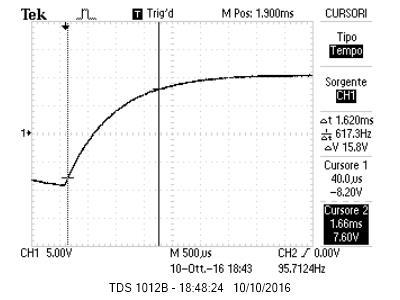
\includegraphics[width=0.5\textwidth]{../oscilloscopio/raise_time.jpg}
	\caption{Tempo di carica del condensatore}
	\label{fig:raise}
\end{figure}

Il valore ottenuto per il tempo di salita del segnale (tra il 10\% e il 90\% del massimo) è $\unit{1.62 \pm 0.06}{\milli\second}$, corrispondente ad una frequenza di $\unit{617 \pm 22}{\hertz}$
%bisogna decidere come stimare l'errore sulla misura del tempo, io userei l'incertezza dei cursori, anche se in realtà mi par di ricordare che la tacca fosse 0.02 ms, mentre per certo 0.1DIV = 0.05 ms, le ho sommate in quadratura

\subsection{Temp:domande teoriche}
%nome temporaneo, decidiamo poi insieme

\section{Filtro passa-banda}

\subsection{I stadio: passa-basso}

\subsection{II stadio: passa-alto}

\subsection{Configurazione a cascata}

\paragraph{Scelta di $R1$ e $R2$} Si poteva scegliere $R1$ e $R2$ in modo che il rapporto fra i due fosse approssimativamente nullo, ad esempio scegliendo $R1$ più piccolo oppure $R2$ più grande.
Infatti il guadagno complessivo può essere scritta come il prodotto dei guadagni dei due stadi per un fattore moltiplicativo. Se $A_1, A_2$ sono i guadagni del primo e del secondo stadio, allora:
\begin{equation*}
A_{tot} = A_1 A_2 \frac{1}{1 + \frac{R_1}{R_2} A_1 A_2}
\end{equation*}


%sui nomi possiamo sempre discutere dopo, per ora sono nomi significativi, se poi per correttezza o estetica vuoi cmabiarli decidiamo insieme
\end{document}
